%% LyX 2.0.2 created this file.  For more info, see http://www.lyx.org/.
%% Do not edit unless you really know what you are doing.
\documentclass[noae]{article}
\usepackage[T1]{fontenc}
\usepackage[utf8x]{inputenc}
\usepackage{geometry}
\geometry{verbose,tmargin=2.5cm,bmargin=2.5cm,lmargin=4cm,rmargin=2.5cm,headsep=0.5cm,footskip=1cm}
\usepackage{amsmath}
\usepackage{amssymb}
\usepackage{graphicx}

\makeatletter

%%%%%%%%%%%%%%%%%%%%%%%%%%%%%% LyX specific LaTeX commands.
%% Because html converters don't know tabularnewline
\providecommand{\tabularnewline}{\\}

%%%%%%%%%%%%%%%%%%%%%%%%%%%%%% Textclass specific LaTeX commands.
\newenvironment{lyxlist}[1]
{\begin{list}{}
{\settowidth{\labelwidth}{#1}
 \setlength{\leftmargin}{\labelwidth}
 \addtolength{\leftmargin}{\labelsep}
 \renewcommand{\makelabel}[1]{##1\hfil}}}
{\end{list}}

%%%%%%%%%%%%%%%%%%%%%%%%%%%%%% User specified LaTeX commands.
\batchmode

\def\input@path{{/home/tran/Bureau/miparcours//}}







%%%%%%%%%%%%%%%%%%%%%%%%%%%%%% LyX specific LaTeX commands.
%% Because html converters don't know tabularnewline
\providecommand{\tabularnewline}{\\}

%%%%%%%%%%%%%%%%%%%%%%%%%%%%%% Textclass specific LaTeX commands.
\newenvironment{lyxlist}[1]{\begin{list}{}
{\settowidth{\labelwidth}{#1}
 \setlength{\leftmargin}{\labelwidth}
 \addtolength{\leftmargin}{\labelsep}
 \renewcommand{\makelabel}[1]{##1\hfil}}}{\end{list}}



\usepackage{Sweave}

\makeatother

\begin{document}

\title{\textbf{Modélisation, Simulation multi-niveau pour l'optimisation
de politiques de vaccination }}


\author{Rapport d'avancement à mi-parcours}


\author{\textbf{TRAN Thi Cam Giang}}


\author{18 Aout 2014}

\maketitle
\textbf{Thesis direction:} Pr. Yann Chevaleyre (PR, Université Paris
13) Dr. Jean-Daniel Zucker (DR1, UMI UMMISCO, IFI-MSI, IRD)

\textbf{Co-supervision:} Dr. Marc Choisy (CR1, MIVEGEC, NIHE, IRD)
Dr. Vu Dinh Thiem (NIHE)


\section{Introduction}

This thesis gives birth in the context where many recent events occur
in the world, for epidemiologie : SRAS in 2003, avian influenza in
2004 or swine flu in 2009, for natural disaster : earthquake -Haiti,
Chile, China-, tsunamis - Indian Ocean in 2004, France in 2010, Japan
in 2011-floods,..., storm insects (cloud of locust), in particular,
infectious disease Ebola being making the entier world worry. These
events have revealed important risks of environment. The rapid spread
of the flu virus recently illustrates how it is important to anticipate
the epidemiological phenomena to better manage when they occur. Moreover,
for vaccination policies, the mass policy (vaccinate the maximum number
of children before certain age) is the oldest (started from the 1950s
in the rich countries) and is now the most used. The problem of this
vaccination policy is too expensive, ineffective and quite impossible
to implement in poor countries, especially in Africa as both financial
and logistical problems. (e.g. the WHO project of extinction measles
in Vietnam before 2012 is failed). Therefore, OPTIMIZE the vaccination
policies in Artificial Intelligence in order that these policies may
become more effective, less expensive, and take into account the spatial
dimension, is the goal of this thesis.

To carry out this goal, the first task is to make a state of the art
covering the different epidemic models being used in the field of
epidemiological modeling. In the second step, we will focus on design
or expand a representation language that allows a modelisator to express
the goals of model simulations as well as constraints related to them.
In the third step, we will set disease population in spatial context,
then study its local/global disease persistence, disease periods and
the influence of space on the disease persistence. Finally, we will
perform vaccination policies in a metapopulation and optimize them.


\section{Epidemic models}


\subsection{State of the art}

We know that, a mathematical model uses the language of mathematics
in order that the description of a system becomes more refined and
more precise. In epidemiology, this model permits us to translate
between behavior at various scales, or extrapolate from a known set
of conditions to another. More robustly, the mathematical models allow
us to predict the epidemic dynamics of population-level, state of
disease under individual as well as under population, spread of disease
and impact of vaccination on the spread of disease infection. These
mathematical models in the epidemiologic field are called the epidemic
models.


\subsubsection{Types of epidemic models}

There are two types of epidemic models : deterministic and stochastic

\textbf{Deterministic}

The deterministic model is described by ordinary differential equations.
It is used in large populations as in the case of infectious disease
such as tuberculosis, mealses, dengue,etc. Here, individuals in the
population are assigned to differents subgroups. Each subgroup represents
a specific stage of the epidemic. The transition rates from one subgroup
to another are derivative equations. The population size in a compartment
is differentiable over time and the epidemic process is deterministic.

\textbf{Stochastic}

``All the disease models that have been considered so far are deterministic''
is the words of Keeling(2008). It means that we have fixed ``clockwork''
processes with the same starting conditions, exactly the same trajectory
is always observed. It isn't right for dynamics of real pathogens
in the real-world. We can not observe exactly the same people becoming
infected at exactly the same times. Therefore, the stochastic model
comes into being. ``Stochastic'' here means having a random variable.
A stochastic model is a tool for estimating probability distributions
of potential outcomes by allowing for random variation in one or more
inputs over time. Or, the stochastic models can be an approximation
or mimicry of this random or probabilistic element. This model has
a important role in special cases, such as when the number of infectious
individuals is rather small, when global extinction is probable to
occur, when the population size is also small and when an infection
has just invaded or is in the trough phase of the epidemic cycle.

\textbf{Terminology}

Here, we give some common terms used in epidemic models. 
\begin{itemize}
\item M : passively immune infants 
\item S : susceptibles 
\item E : exposed individuals in the latent period 
\item I : infectives 
\item R : removed with immunity 
\item $\beta$ : contact rate such that a susceptible becomes an infectived 
\item $\lambda$ : infection rate 
\item $\mu$ : average death rate and at the same time, average birth rate 
\item $\sigma$ : average rate of the latent period 
\item $\gamma$ : average rate of the infectious period 
\item N : population size 
\end{itemize}

\subsubsection{Epidemic models}

At present, there are many epidemic models. We can divide these models
into two base types, the type of three base elements and the type
of more than three base elements.

\textbf{Epidemic models with three base elements:}

We have the SIR model, the SIR model with births and deaths, the SIS
model with births and deaths, and the SIRS model. The first simplest
model is the SIR model created by W. O. Kermack and A. G. McKendrick
in 1927. The model is fixed with three elements: susceptible S(t),
infected I(t) and removed R(t). These three elements are correspondant
to its three classes. From the simplest SIR model, in order to accord
each infectious disease and real property of disease, scientists have
modified it, make it more multiforme. For example, for SIS models,
the individuals recover with no immunity to the disease, that is,
inviduals are immediately susceptible once they have recovered. This
SIS models are used in sexually transmitted diseases like gonorrhoea
because once recovered, the host is once again susceptible to infection.

\textbf{Epidemic models with more than three base elements:}

Here, we also have a lot of epidemic models with more than three base
elements, to accord many different disease types, such as the SEIS
model, SEIR model, MSIR model, MSEIR model and MSEIRS model. However,
in shape of this thesis, we concentrate on the SEIR model (as the
figure \ref{fig:seirmodel})that consists with many currently infectious
diseases in the world. Diseases have a latent or exposed phase, during
which the individual is said to be infected but not infectious.

\begin{figure}[tbph]
\centering 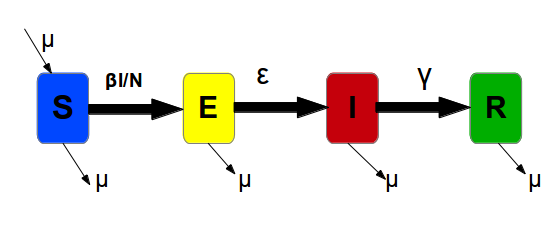
\includegraphics[width=0.5\textwidth]{seirmodel} \caption{SEIR model}


\label{fig:seirmodel} 
\end{figure}


In this model, the host population (N) is divided into four classes
: susceptible S(t), exposed E(t), infected I(t) and recovered R(t).
We have :

$N=S(t)+E(t)+I(t)+R(t)$ 
\begin{itemize}
\item Classe S(t) : contains the number of individuals not yet with the
disease at time t, or those susceptible to the disease. 
\item Classe E(t) : contains the number of individuals who are in the exposed
or latent period of the disease. 
\item Classe I(t) : contains the number of individuals who have been infected
with the disease and are capable of spreading the disease to those
in the susceptible category. 
\item Classe R(t) : contains the number of individuals who have been infected
and then removed from the disease, either due to immunization or due
to death. Individuals of this classe are not able to be infected again
or to transmit the disease infection to others. 
\end{itemize}

\subsection{Demographic stochasticity}

Demographic stochasticity is still called event-driven stochasticity,
because it is built upon events. This stochasticity is considered
as fluctuation in population process that arise from random differences
among individuals. Therefore, demographic stochasticity becomes a
common tool of scientists to epidemics model due to its mechanistic
approach to including randomness and the individual nature of its
formulation. The number of infectious, susceptible, exposed and recovered
individuals in a population must here be integers.

In short, in demographic stochasticity, there are two elements in
common, one is event and the other is random number. The first algorithm
\textquotedbl{}First Reaction Method'' is born in 1976 by Gillespie.
Then, based on this first algorithm and these two key elements of
demographic stochasticity, many scientists improved the first method,
and created many better algorithms for stochastic simulations. But
typically, there are only two main types of algorithms, exact algorithms
and approximative algorithms. The typical algorithm that most practitioners
use, among exact algorithms, is the algorithm ``Direct Method''
of Gillespie(1977) improved from the first algorithm ``First Reaction
Method'', and among approximative algorithms, is the ``tau-leaping''
algorithm. With these two types of algorithms, each has its private
advantages and its private disadvantages. They have a common point.
Their processes are in continuous-time Markov process for which the
transition rates are constants, isn't a function of time. The future
state of the process, is only conditional on the present state, but
independent of the past. In constract, privately, for the exact algorithm,
its advantage give us a really exact approach of simulating population-based
time-to-event through two step with many iterations of 1) searching
the time of next event by an exponentially distributed function and
2) searching the nature of next event. This process is repeated to
iterate the model. In addition to the exact algorithms, Gibson \&
Bruck (2000) modified the first reaction method and created the Next
Reaction method that substantially more challenging to program but
is significantly faster than even the method when there are a large
number of different event types. The Direct, First Reaction and Next
Reaction methods are all exact stochastic approaches of the underlying
ODEs. For these exact methods, on the one hand, noise in simulation
only affects the probabilities associated with fates of individuals
and the updating of each consecutive event is independent – there
is no assumption concerning environmental stochasticity. On the other
hand, these exact solutions become too slow and impractical when any
one transition rate is large, when there is a big number of subpopulations
or one a big number of event in a metapopualtion. It is the reason
for that, approximate models are born instead of the exact stochastic
methods. Gillespie (2001) has proposed a new method that decreases
the simulation accuracy, but increases simulation speed. This is the
``$\tau-leap$ method'' known as an approximate method reduces the
number of iterations by treating transition rates as constant over
time periods for which this approximation leads to little error \cite{KeelingRohani2008}.
View the figure \ref{fig:speed}. 
\begin{figure}[tbph]
\centering 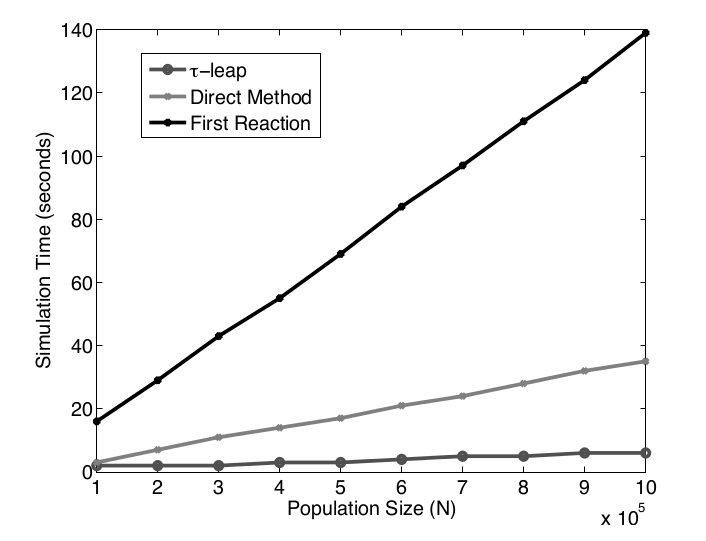
\includegraphics[width=0.5\textwidth]{speed} \caption{Figure is extrait from Keling (2008) The time (in seconds) to simulate
1000 years of SEIR epi- demics ($\mu=0.02$ per year, $1/\sigma=8$
days, $1/\gamma=10$ days) on a 3.4GHz Pentium PC. For Gillespie’s
Direct (light grey line) and First Reaction (black line) methods,
as the population size increases so does the simulation time, which,
for very large populations, could become prohibitive. In contrast,
the ``$\tau-leap$ method (dark grey) is fast and largely unaffected
by population size \cite{KeelingRohani2008}. }


\label{fig:speed} 
\end{figure}



\subsubsection{Disease transmission types in epidemic models }

We know that, for each disease, knowing well its transmission methods
is important for implementing proper infection control measures and
prevention campaigns with large scale. The disease transmission methods
depend on the characteristics of each disease and the nature of the
microorganism that causes it. Here, we will point out some main types
of transmission. For some infectious disease, its transmission method
is complex and variant, such as anthrax. The anthrax can be spread
through direct contact to a cut on the skin or through airborne spores
which are inhaled. 
\begin{lyxlist}{00.00.0000}
\item [{\textbf{Transmission}}] \textbf{by direct contact} 
\end{lyxlist}
This transmission requires a close contact between an infected person
and a susceptible person, such as touching an infected individual,
kissing, sexual contact, contact with oral secreations, or contact
with body lesions. Therefore, disease usually occurs between members
of the same household or close friends and family. 
\begin{lyxlist}{00.00.0000}
\item [{\textbf{Transmission}}] \textbf{by indirect contact} 
\end{lyxlist}
The indirect transmission has an intermediate factor where a susceptible
person can be infected by a contaminated surface. The touch surfaces
are usually in the life : door knobs, door handles; tables, beds,
chairs; washroom surfaces; cups, dishes, trays; medical instruments;
children's toy, etc. So, in order to reduce the number of infected
individuals, we always make frequent touch surfaces be properly disinfected. 
\begin{lyxlist}{00.00.0000}
\item [{\textbf{Transmission}}] \textbf{by droplet contact} 
\end{lyxlist}
These droplets are infected droplets that we usually see on the eye,
nose and mouth. Droplets containing microorganisms can spread diease
when an infected person coughs, sneezes and talks or through medical
procedures. Droplets are too large to be airborne for long periods
of time, and quickly settle out of air. We know measles and SARS are
two exemples of transmission with droplet transmission. However, to
reduce the infection, we can take personal protective barriers such
as face masks and googgles to prevent disease transmission. 
\begin{lyxlist}{00.00.0000}
\item [{\textbf{Transmission}}] \textbf{by airborne} 
\end{lyxlist}
This is quite dangerous cas where droplets are dust particles containing
microorganisms. These organisms can remain suspended in air for long
periods of time. And we become infected when we inhale these organisms.
Fortunately, only a limited number of diseases are capable of airborne
transmission, such as tuberculosis, chickenpox and measles. 
\begin{lyxlist}{00.00.0000}
\item [{\textbf{Fecal-oral}}] \textbf{transmission} 
\end{lyxlist}
Fecal-oral transmission is usually associated with organisms that
infect the digestive system, through ingestion of contaminated food
and water. Fecal-oral transmission can be reduced by 
\begin{itemize}
\item Proper storage of food at proper temperatures 
\item Thorough cooking of food 
\item Frequent and thorough handwashing, especially after washroom use 
\item Adequate sewage treatment and water filtration/chlorination systems 
\item Disinfection of frequent touch surfaces to prevent indirect contact
transmission 
\item Increased public awareness of proper hygiene and food handling 
\end{itemize}
\textbf{Vector-borne transmission}

Vectors are animals that are capable of transmitting diseases, such
as flies, mites, fleas, ticks, rats, dogs, and in particular, mosquito.
Since vectors are mobile, they increase the transmission range of
a disease. So, changes in vector behaviour will affect the transmission
pattern of a disease. It is important to study the behaviour of the
vector as well as the disease-causing microorganism in order to establish
a proper method of disease prevention. 
\begin{lyxlist}{00.00.0000}
\item [{\textbf{Others}}] ~ 
\end{lyxlist}
In addition to the transmission due to\textbf{ }the characteristics
of each disease and the nature of the microorganism, we also study
demographic factors as the following: 
\begin{itemize}
\item Age-structured populations 
\item Variable infectivity 
\item Distributions that are spatially non-uniform 
\item Diseases caused by macroparasites 
\item Acquired immunity through vaccination 
\end{itemize}

\section{Approaches in use}

In the shape of this thesis, we use the most general SEIR model for
infectious diseases, feature as diseases with transmission by airborne,
such as meales that the entier world in the beginning of the 2014
was quite interrested. The World Health Organization (WHO) had officially
to state global measles epidemic outbreak. In the first three months
of the year 2014, there were about 56,000 cases of measle infections
in 75 countries \cite{WHO2014a}, in particular in southeast Asia
particularly, in Vietnam \cite{http://healthmap.org/site/diseasedaily/article/measles-reemerges-vietnam-22814}.
Moreover, in this thesis, we will introduce the SEIR model for many
subpopulations in a metapopulation.


\subsection{Deterministic model for many cities}


\subsubsection{Ordinary differential equations for the deterministic model of many
cities}

The standard SEIR model (susceptible-exposed-infective-recovered)
has been strongly developped for the dynamics of directly infectious
disease \cite{Bolker1995}. For disease-based metapopulation models,
we give here a suitable new version of the SEIR equation that would
be as follows:

Consider a metapopulation of $n$ sub-populations. In a subpopulation
$i$ of size $N_{i}$, disease dynamics can be deterministically described
by the following set of differential equations \cite{Anderson&May1992}:

\begin{eqnarray}
\frac{dS_{i}}{dt} & = & \mu N_{i}-\lambda_{i}S_{i}-\mu S_{i}\label{eq:dS}\\
\frac{dE_{i}}{dt} & = & \lambda_{i}S_{i}-\mu E_{i}-\sigma E_{i}\\
\frac{dI_{i}}{dt} & = & \sigma E_{i}-\mu I_{i}-\gamma I_{i}\label{eq:infectieux}\\
\frac{dR_{i}}{dt} & = & \gamma I_{i}-\mu R_{i}\label{eq:dR}
\end{eqnarray}
 where $S_{i}$, $E_{i}$, $I_{i}$ et $R_{i}$ are the numbers of
susceptible, exposed, infectious and recovered in this sub-population
$i$ respectively. Individuals are born susceptible, die at a rate
$\mu$, become infected with the force of infection $\lambda_{i}$,
infectious after a latency period of an average duration of $1/\sigma$
and recover at the rate $\gamma$.


\subsubsection{Formula for force of infection}

The force of infection depends not only on the total population size
$N_{i}$ and the number of infected $I_{i}$ in subpopulation $i$,
but also in other sub-populations \cite{KeelingRohani2008}.

\begin{equation}
\lambda_{i}=\beta_{i}\frac{I_{i}}{N_{i}}+\sum_{\substack{j=1\\
j\neq i
}
}^{n}\rho_{ij}\left[\frac{\beta_{i}\text{[}(1-\varepsilon_{ij})I_{j}-I_{i}]}{N_{i}}+\frac{\varepsilon_{ij}\beta_{j}I_{j}}{N_{j}}\right]\label{eq:force-1}
\end{equation}
 where $\beta_{i}$ is the contact rate in population $i$ and $\rho_{ij}=\rho_{ji}$
($0\leqslant\rho_{ij}\leqslant1$ and $\rho_{ii}=1$) is the coupling
between subpopulations $i$ and $j$. Among the infections caused
by contacts with infected from other subpopulations, $\varepsilon_{ij}=\varepsilon_{ji}$
($0\leqslant\varepsilon_{ij}\leqslant1$) is the proportion of infections
due to susceptible individuals visiting other populations as opposed
to infected individuals from other populations visiting the focal
population. See appendix for detail on the construction of this equation.
We can verify that in the limit case on one single subpopulation in
the metapopulation ($i=j$ and $n=1$) we have 
\begin{equation}
\lambda_{i}=\beta_{i}\frac{I_{i}}{N_{i}}.
\end{equation}
 Consider that the contact rate $\beta_{i}$ is seasonally forced
\cite{Altizer2006} and seasonality is an annually periodic function
of time \cite{Grenfell1995}. As a result, 
\begin{equation}
\beta_{i}(t)=b_{0}\left[1+b_{1}\cos\left(\frac{2\pi t}{T}+\varphi_{i}\right)\right]\label{eq:beta_i}
\end{equation}
 where $t$ is the time, $b_{0}$ and $b_{1}$ are the mean value
and amplitude of the infection rate $\beta$ at which susceptible
individuals become infected, $T$ and $\varphi_{i}$ are the period
and the phase of the forcing. With the annual sinusoidal form of the
infection rate, we really have the sinusoidally forced SEIR metapopulation
model.


\subsubsection{Equilibrium values of the system}

In a case the infectious contact rate is constant, the equilibrium
values of the variables $S$, $E$, $I$ and $R$ can be expressed
analytically as follows. We know that, in simulation, the equilibrium
state allow a disease to persist in a population for a long time.
So, an infectious disease in the $subpopulation_{i}$ is available
in long term this system is at equilibrium. It means that at which
$\frac{dS_{i}}{dt}=\frac{dE_{i}}{dt}=\frac{dI{}_{i}}{dt}=\frac{dR{}_{i}}{dt}=0$
({*}). Thus, we let all equations (equations $1$ - $4$ ) in the
system be equal to zero, then calculate the values of the variables
(now denoted by $S_{i}^{*}$, $E_{i}^{*}$, $I_{i}^{*}$ , and $R{}_{i}^{*}$)
that satisfy this condition ({*}). We have these values as folllows:

\begin{eqnarray}
S_{i}^{*} & = & N_{i}\frac{(\gamma+\mu)(\sigma+\mu)}{\beta\sigma}\\
E_{i}^{*} & = & N_{i}\mu\left(\frac{1}{\sigma+\mu}-\frac{\gamma+\mu}{\beta\sigma}\right)\\
I_{i}^{*} & = & N_{i}\mu\frac{\beta\sigma-(\sigma+\mu)(\gamma+\mu)}{\beta(\sigma+\mu)(\gamma+\mu)}\\
R_{i}^{*} & = & N_{i}-S_{i}^{*}-E_{i}^{*}-I_{i}^{*}
\end{eqnarray}


Here, if we set $R_{0}=\frac{\beta\sigma}{(\gamma+\mu)(\sigma+\mu)}$,
so we have

\begin{eqnarray}
S_{i}^{*} & = & N_{i}\frac{1}{R_{0}}\\
E_{i}^{*} & = & N_{i}\frac{\mu\sigma}{R_{0}}\left(R_{0}-1\right)\\
I_{i}^{*} & = & N_{i}\frac{\mu}{\beta}(R_{0}-1)\\
R_{i}^{*} & = & N_{i}-S_{i}^{*}-E_{i}^{*}-I_{i}^{*}
\end{eqnarray}


One nomal conditions for all population availabes is that the equilibrium
values cannot be negative. Therefore, an infectious disease is available
in the $subpopulation_{i}$ if $R_{0}>1$. Now, the endemic equilibrium
in the system is given by $(S_{i}^{*},E_{i}^{*},I{}_{i}^{*},R{}_{i}^{*})$
= $(N_{i}\frac{1}{R_{0}}$, $N_{i}\frac{\mu\sigma}{R_{0}}\left(R_{0}-1\right)$,
$N_{i}\frac{\mu}{\beta}(R_{0}-1)$, $N_{i}(1-\frac{1}{R_{0}}-\frac{\mu\sigma}{R_{0}}\left(R_{0}-1\right)-\frac{\mu}{\beta}(R_{0}-1))$.


\subsection{Stochastic model for many subpopulation in a metapopulation}


\subsubsection{Stochastic model for many subpopulations in a metapopulation}

In order to study the persistence of the disease, we must consider
a stochastic version of the model \cite{Keeling2002,Lloyd2001,renshaw1993modelling}.
We use for that a population-based time-to-next-event model based
on Gillespie's algorithm \cite{gillespie1977exact}. Table \ref{tab:stoch_ev}
lists all the events of the model, occurring in subpopulation $i$.

\begin{table}[tbph]
\begin{centering}
\caption{\label{tab:stoch_ev}Events of the stochastic version of the model
of equations \ref{eq:dS}-\ref{eq:dR}, occuring in subpopulation
$i$.}

\par\end{centering}

\centering{}%
\begin{tabular}{lcc}
\textbf{Events}  & \textbf{Rates}  & \textbf{Transitions} \tabularnewline
birth  & $\mu N_{i}$  & $S_{i}\leftarrow S_{i}+1$ and $N_{i}\leftarrow N_{i}+1$ \tabularnewline
death of a susceptible  & $\mu S_{i}$  & $S_{i}\leftarrow S_{i}-1$ \tabularnewline
death of an exposed  & $\mu E_{i}$  & $E_{i}\leftarrow E_{i}-1$ \tabularnewline
death of an infected  & $\mu I_{i}$  & $I_{i}\leftarrow I_{i}-1$ \tabularnewline
death of an immune  & $\mu R_{i}$  & $I_{i}\leftarrow I_{i}-1$ \tabularnewline
infection  & $\lambda_{i}S_{i}$  & $S_{i}\leftarrow S_{i}-1$ and $E_{i}\leftarrow E_{i}+1$ \tabularnewline
becoming infectious  & $\sigma E_{i}$  & $E_{i}\leftarrow E_{i}-1$ and $I_{i}\leftarrow I_{i}+1$ \tabularnewline
recovery  & $\gamma I_{i}$  & $I_{i}\leftarrow I_{i}-1$ and $R_{i}\leftarrow R_{i}+1$ \tabularnewline
 &  & \tabularnewline
\end{tabular}
\end{table}



\subsubsection{Exact method for many subpopulations in a metapopulation}

As pointed out above, the direct method is usually more computationally
efficient. This is the exact stochastic method more commonly used
of the underlying ODEs. However, this method is only proposed for
one population, so here we modify a little the direct method in order
to accord with a metapopulation of multi-subpopulation. We call it
``the direct method of multi-subpopulation''. View the figure \ref{fig:exactGil}.

This multi-subpopulation method add two steps into the direct method,
these are steps 3 and 4. We generate one more new random number, and
then we convert population rates into probabilities, finally this
new random number is used to select one of the subpopulation in the
metapopulation of $n$ subpopulations.

\begin{figure}[tbph]
\centering 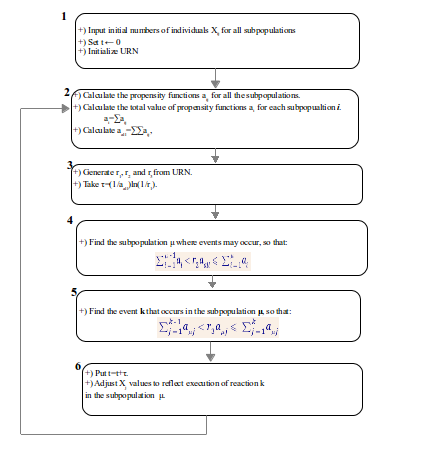
\includegraphics[width=0.5\textwidth]{exactGil} \caption{Improving the exact algorithm of Gillespie (1977) for a metapopulation
of multi-subpopulation.}


\label{fig:exactGil} 
\end{figure}



\subsection{Result}


\subsubsection{Package \textquotedbl{}dizzys'' for stochastic SEIR metapopulation
model}

At present, we built successfully a package named ``dizzys''. This
package in R implements both the exact and approximate methods for
the deterministic/stochastic SEIR/SIR models by integrating the R
package and the C++ implementation. We use C++ to perform the algorithms,
and use R to create interfaces. Hence, this new integration is faster
than any pure R implementation.

\textbf{Simulation 1:}

Simulating the deterministic and stochastic SEIR model for one seul
population. View the figure \ref{fig:smDetSto}.

\begin{figure}[htpb]
\centering 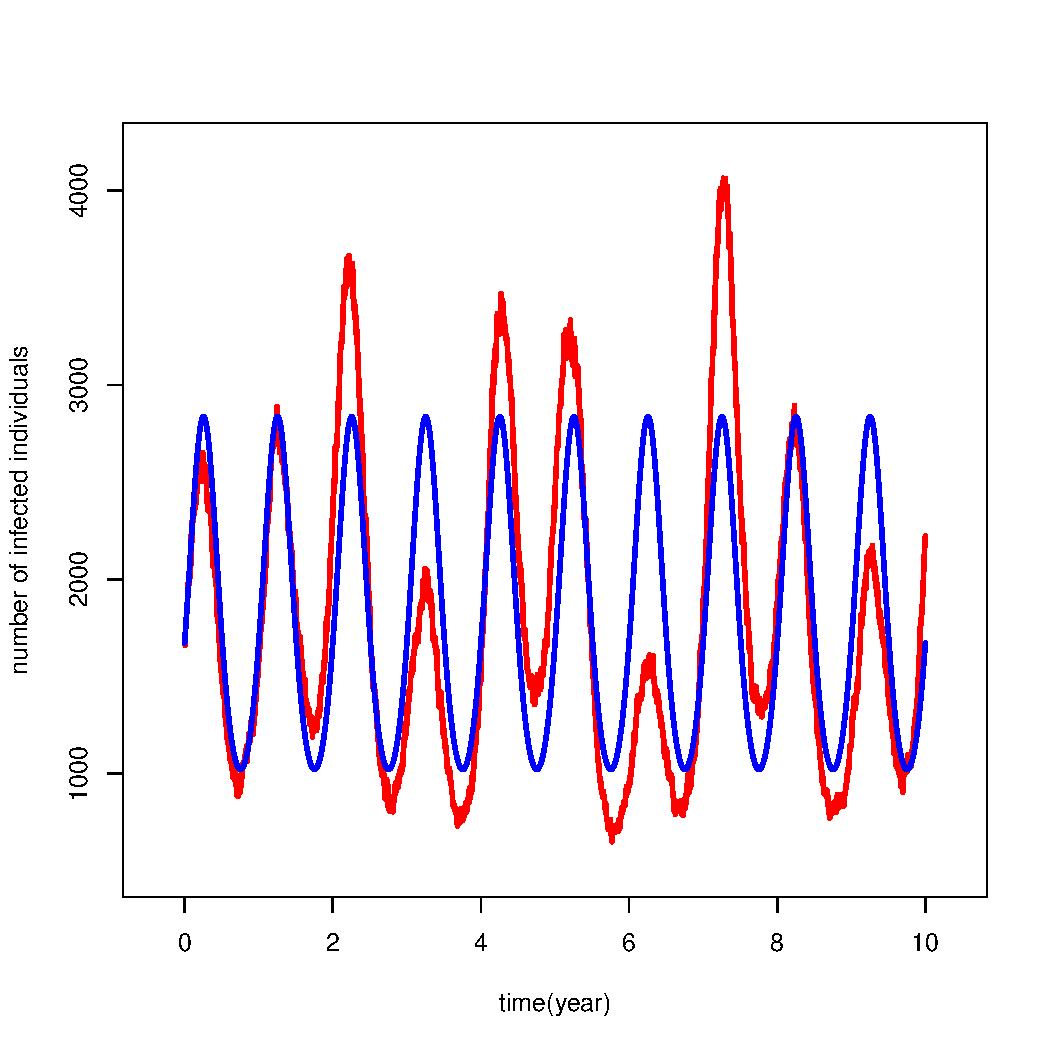
\includegraphics[width=0.5\textwidth]{smDertSto} \caption{\label{fig:smDetSto}Deterministic/stochastic SEIR model for one seul
population with N=$10^{7}$, duration=10year. The blue fluctuation
for the deterministic model and the red for the stochastic model.}
\end{figure}


\textbf{Simulation 2:}

Simulating three subpopulations with the different population sizes,
then continuing or redoing this simulation with other values of parameter,
we can do it by exploiting the 'simul' function in the package. View
the figure \ref{fig:multiSub}.

\begin{figure}[tbph]
\centering 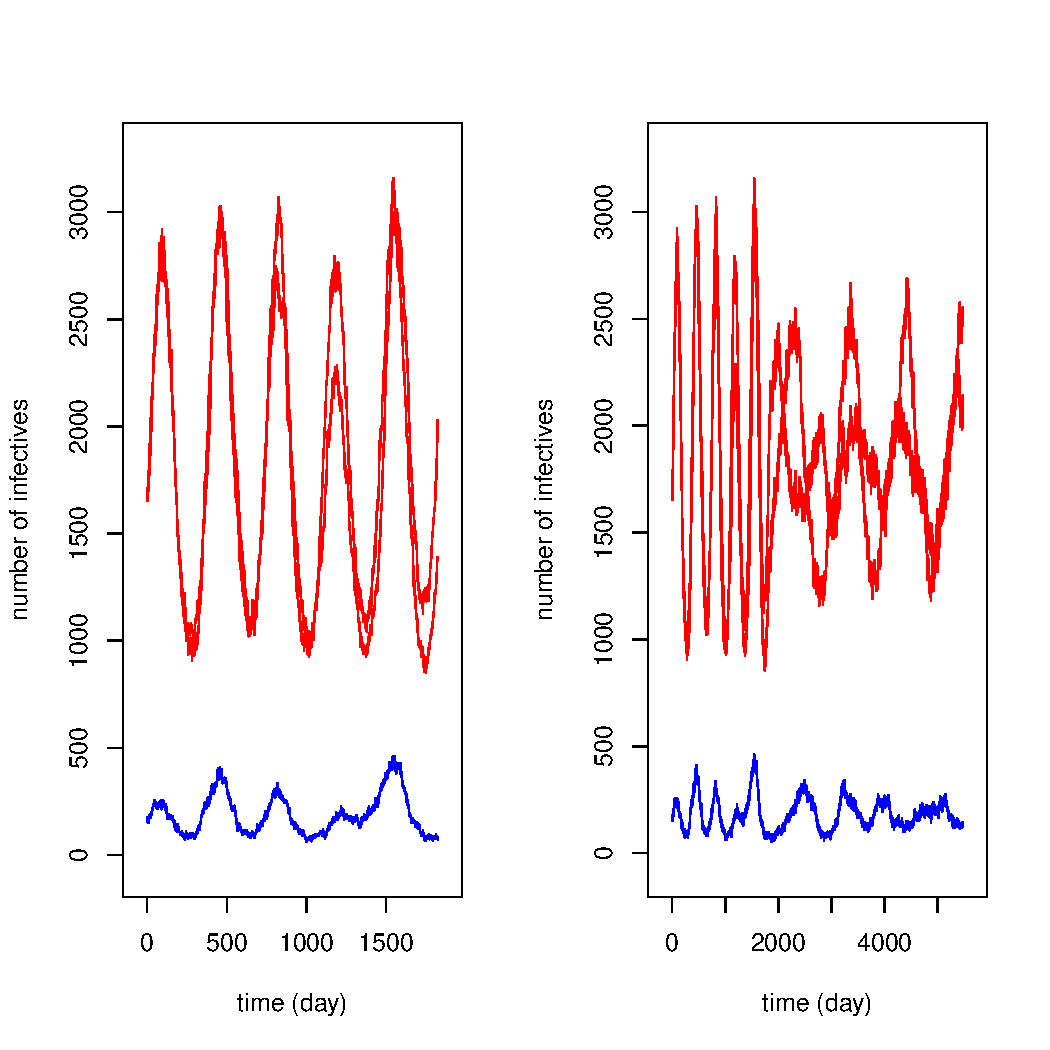
\includegraphics[width=0.5\textwidth]{mulSubpop} \caption{Continuing or redoing this simulation. The start seir object with
type=\textquotedbl{}stochastic\textquotedbl{}, duration=5{*}365, mu=1/(70{*}365),
beta0=1000/365, beta1=.1, sigma=1/8, gamma=1/5, nbVilles=3, N=c($10^{7}$,$10^{6}$),
phi=0, duration=5{*}365; and the last seir object with type=\textquotedbl{}stoch\textquotedbl{},
continue=T, append=T, beta1=0.0, phi=pi, duration=10{*}365. The two
red fluctuations for the two first subpopulations with N=$10^{7}$
and the blue for the third subpopulation with N=$10^{6}$}


\label{fig:multiSub} 
\end{figure}


\textbf{Simulation 3:}

The SEIR stochastic model using ``adaptive tau-leaping'' algorithm
by exploiting the function ``simul'' in the package. To do this
algorithm, we only make the parameter $method="adaptivetau"$. We
can compare the result of the direct algorithm with the result of
the adaptivetau algorithm as follows. View the figure \ref{fig:smDrectAdap}.

\begin{figure}[tbph]
\centering 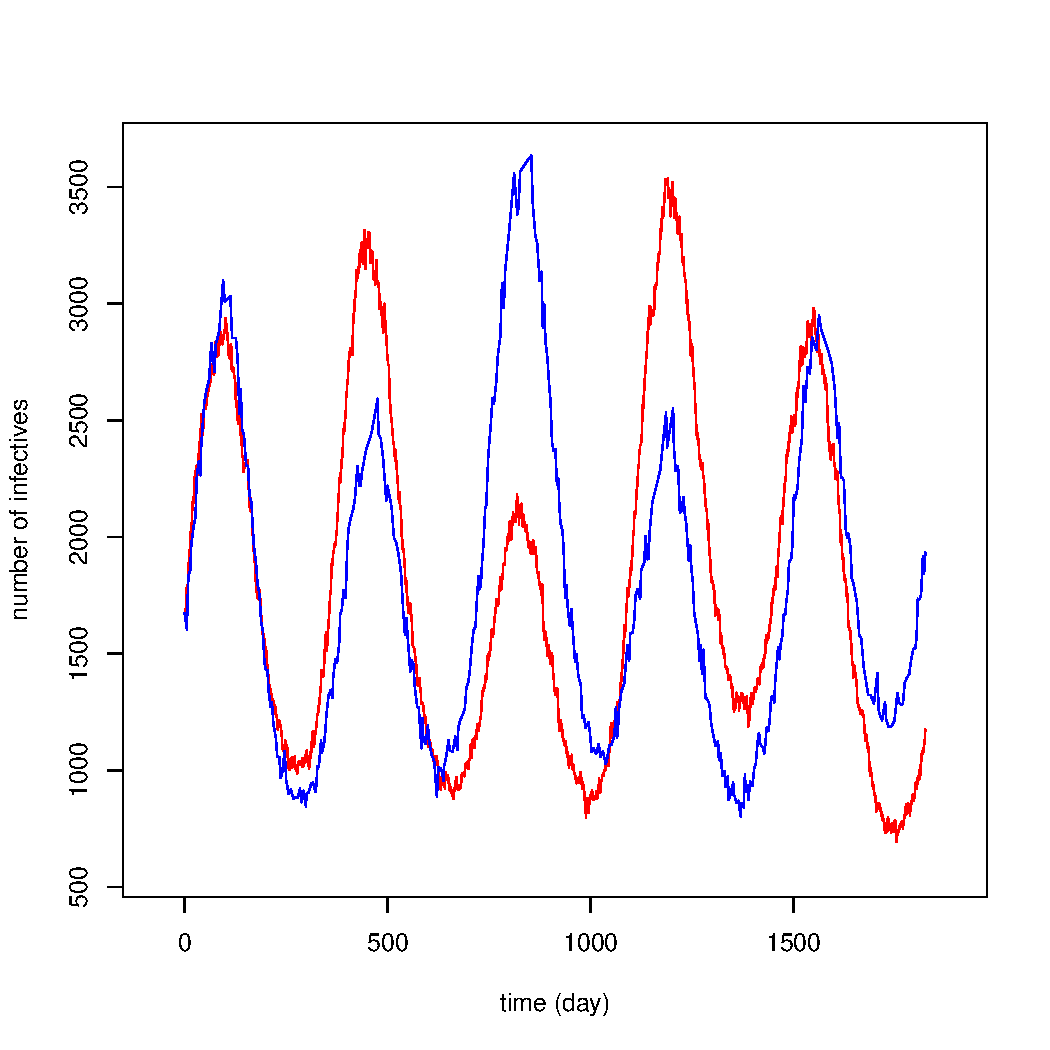
\includegraphics[width=0.5\textwidth]{compDirectAdap}
\caption{Compare the result of the direct algorithm with the result of the
adaptivetau algorithm. The red fluctuation for the direct method and
the blue for the \textquotedbl{}$\tau$ - leap'' method.}


\label{fig:smDrectAdap} 
\end{figure}


Simulation 4:

Plot in 3D, view the figure \ref{fig:plot3D}.

\begin{figure}[tbph]
\centering 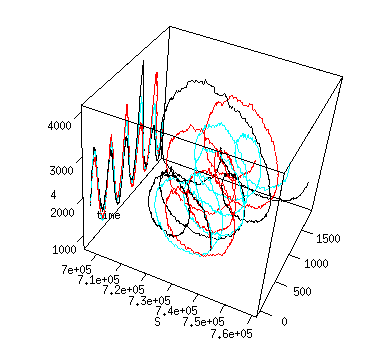
\includegraphics[width=0.5\textwidth]{plot3D} \caption{Plot in 3D of the stochastic SEIR model with the three subpopulations
in the metapopulation. We view the relation between the number of
susceptible individuals, the number of infected individuals and the
time. Then, we can also view the projection of these fluctions on
the correspondent surface.}


\label{fig:plot3D} 
\end{figure}



\subsubsection{Global persistence in a metapopulation}

Here, we start exploiting the package \textquotedbl{}dizzys''. In
order to illustrate the interaction between disease transmissibility
and phase of seasonal forcing, we start in this section by studing
the stochastic SEIR model in a metapopualtion of $n$ subpopulations.
For this meta-population, we observe the disease extinction in time
due to spatial synchrony or spatial asynchrony that are influenced
by phase difference in seasonal forcing. To create the phase difference,
we change the value of the forcing phase for each city. In this experience,
we use a parameter $\varphi_{max}$ in radian that runs in the interval
from zero to $\pi$. With each value of $\varphi_{max}$, based on
\textbf{$n$} the number of subpopulations in the metapopulation,
we divide the interval {[}0, $\varphi_{max}${]} into a set of (n-1)
equal samples, so the value of the forcing phase of the $i^{th}$
city is correspondent to $i^{th}$ value in the set. We call $\varphi_{max}$
synchrony parameter.

For our metapopulation of $n$ subpopulations, to do so we run first
$m$ independent simulations of our stochastic model. We calculate
then the average metapopulation size by summing subpopulations at
each sample time and averaging across the entire time series for each
metapopulation. Lastly, we record the dates $t$ of global disease
extinction in all these $m$ metapopulations. These dates allowed
to draw Kaplan-Meier survival curves from which we estimated the persistence
rates $\chi$: 
\begin{equation}
M(t)=\exp(-\chi t)
\end{equation}
 where $M(t)$ ($0\leqslant M(t)\leqslant m$) is the number of metapopulations
in which the disease is not extinct at time $t$.

To estimate the persistence rate, here, we use the parametric survival
model for the exponential distribution (R package '$survival$' \cite{survival-package}).
For that, we find the persistence rate of the number of metapopulations
in which the disease is extinct in time. Based on this persistence
rate, we study the relation between the global persistence and its
average synchrony due to the phase of the forcing.


\paragraph{Global persistence and time}

We fixe here the metapopulation of two subpopulations, $N_{1}=N_{2}=300,000$,
the rate of coupling $\rho=0.01$, the simulation time 50 years, the
number of simulations $m=100$, and $\varphi_{max}=\{0,\pi/2,\pi\}$.
Now, we have 100 metapopulations, we gather the first time where the
metapopualtion gets global extinction. We have three Kaplan-Meier
survival curves for each value of $\varphi_{max}$ as figure \ref{fig:persm100phi0pi2pi_01}.

\begin{figure}[tbph]
\centering 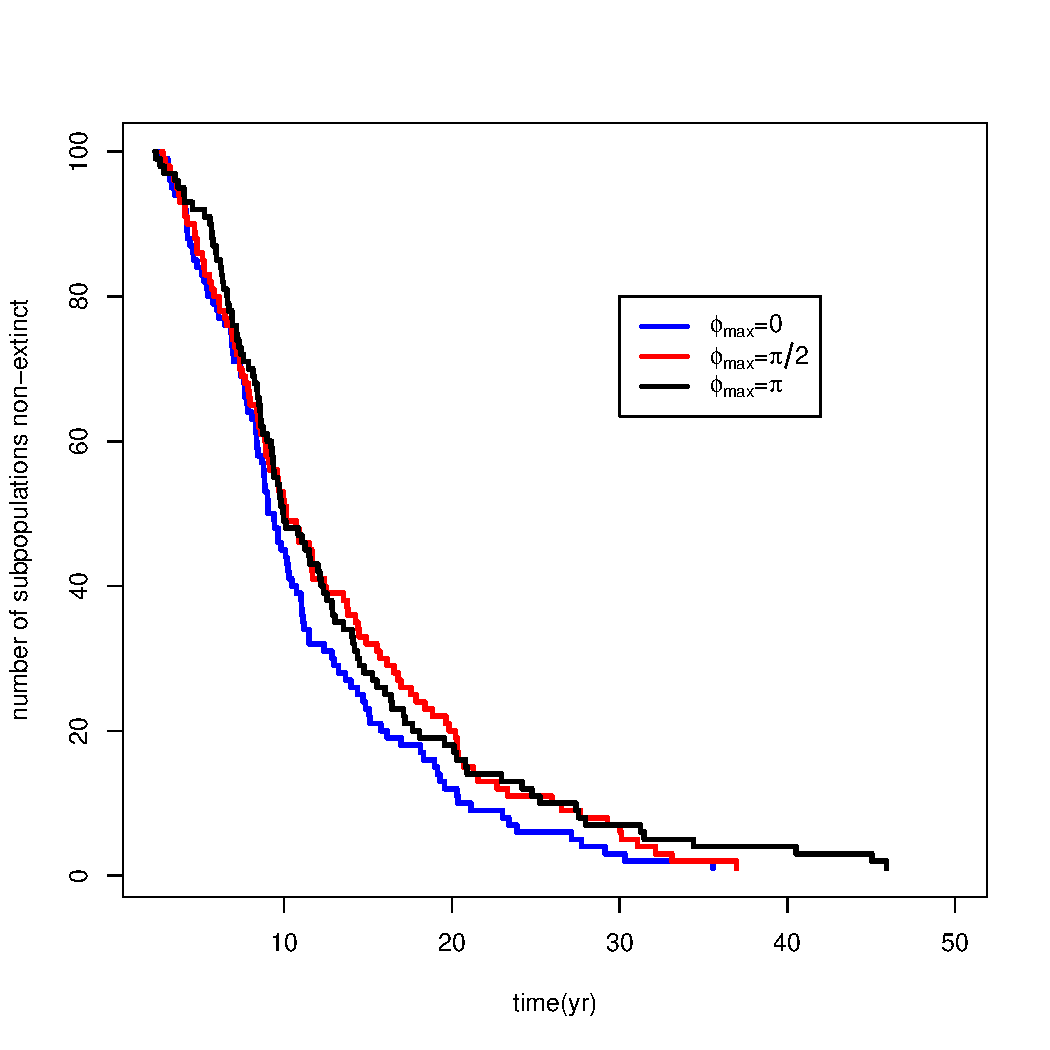
\includegraphics[width=0.5\textwidth]{smRep100Vil02R001N3e5}
\caption{Kaplan-Meier survival curves for disease persistence after 100 different
simulation\protect \protect \protect \\
 Disease persistence time after 100 simulations of $\varphi_{max}=0$,
$\varphi_{max}=\pi/2$ and $\varphi_{max}=\pi$. The blue survival
curve for $\varphi_{max}=0$, the red survival curve for $\varphi_{max}=\pi/2$
and the black curve for $\varphi_{max}=\pi$. The persistence time
of $\varphi_{max}=0$ is the shortest. The persistence time of $\varphi_{max}=\pi$
is the longest.}


\label{fig:persm100phi0pi2pi_01} 
\end{figure}


The phase of forcing of the $subpopulation_{1}$ is always fixed $0$,
but this of the $subpopulation_{2}$ increases from $0$ to $\pi$.
It means that, in the first experience, $\varphi_{max}=0$, the two
subpopulations are in synchrony with all beginning conditions. The
disease persistence time is the shortest. Then, the two subpopulations
become asynchrony when $\varphi_{max}=\pi/2$ or $\pi$. The symmetry
of fixed points is just broken at the starting moment. It is reason
for that the level of synchrony of the metapopulation decreases. Additionally,
we find that the value of the synchrony parameter $\varphi_{max}$
change according to increasing tendency, the phase difference between
the fluctuations of the two infection rates $\beta$ increases also,
and the global persistence time in the metapopulation thus augments.
When \textbf{$\varphi_{max}=\pi$, }the two subpopulations are in
antiphase. This is the most difficult case to find global extinction,
the persistence time is the longest. In short, the level of synchrony
between subpopulation is stronger, metapopualtion is easier to find
global extinction. Make all subpopulations synchronize is the easiest
way at which disease goes to extinct.


\paragraph{Global persistence rate and $\varphi_{max}$}

In this part, the Kaplan-Meier survival curves of the global disease
persistence time in a metapopulation for each value $\varphi_{max}$
is considered as a parameter that is called global persistence rate
of that $\varphi_{max}$. We used survival functions to estimate this
global persistence rate with confidence interval 95\%. The result
is shown as following figure \ref{fig:perrateVil2}.

\begin{figure}[tbph]
\centering 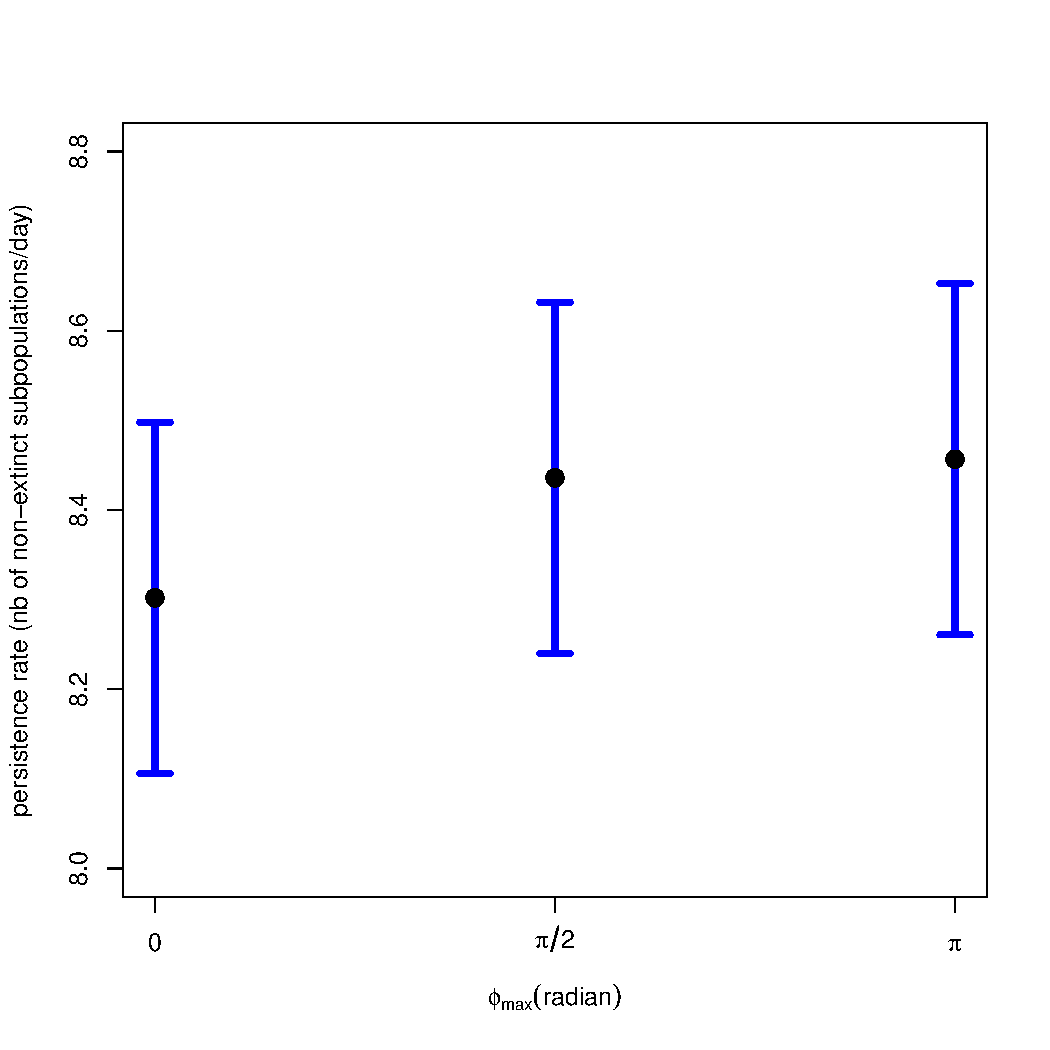
\includegraphics[width=0.5\textwidth]{resPop02Rho001N3e5Rep100}
\caption{Estimated rate of global disease persistence in the metapopulation
of the two subpopulations after 100 different simulations N=3e5, coupling
rate $\rho=0.01$. Here, with 95\% confidence interval, blue lines
are confidence intervals for persistence rate of each value of $\varphi_{max}$.
This intervals are limited by lower and upper confidence limits.}


\label{fig:perrateVil2} 
\end{figure}


This figure \ref{fig:perrateVil2} points out to us that the amplitude
of the confidence intervals for each value of $\varphi_{max}$ are
quite close to each other. However, it gradually rises when $\varphi_{max}$
runs from $0$ to $\pi$. The phase difference strongly influences
disease persistence time, at the same time, global disease persistence
rate. The asynchrony between subpopulaitons is the main reason to
respond very familiar question why has the infectious disease been
never extinct.

\begin{figure}[tbph]
\centering 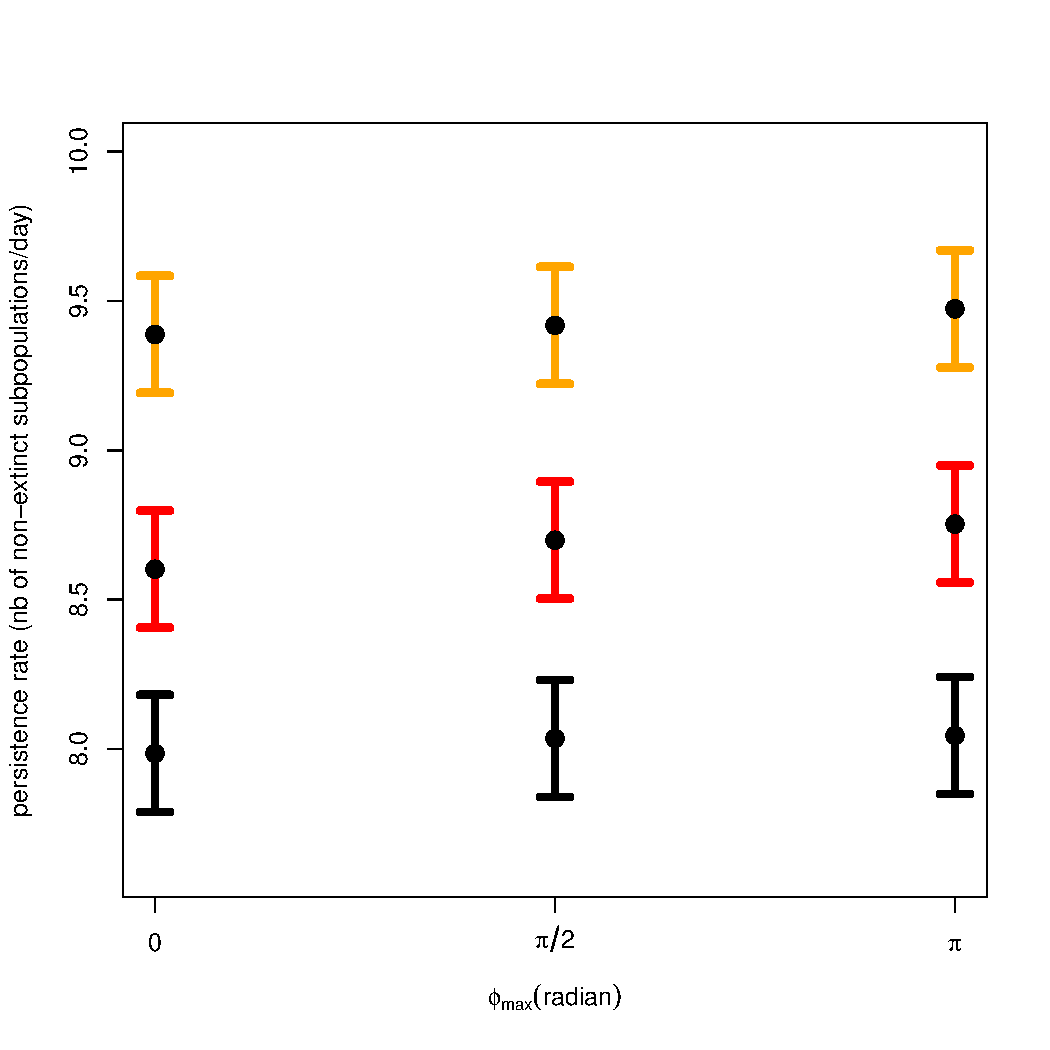
\includegraphics[width=0.5\textwidth]{resVil3510Rho0001N2e5}
\caption{Estimated persistence rate in the metapopulation of three, five and
ten subpopulations after 100 different simulations. Here, with 95\%
confidence interval, black, red, and orange lines are for three, five
and ten subpopulations, respectively. These intervals are limited
by lower and upper confidence limits. }


\label{fig:confintVil3510Rho0001N2e5} 
\end{figure}


One more factor that was pointed in this introduction part is coupling
strength between subpopulations. We can say that this coupling parameter
can symbolize migration strength. The disease transmission speed fast
augments when coupling rate goes up in metapopulation. Similar to
that, global disease persistence increases also. Here, we permit coupling
rate change from weak to strong in a metapopualtion of five subpopulations
with $N=10^{5}$ for each subpopulation. The dispersal rate $\rho$
is divised into three intervals. These are low, intermediate and high
coupling rate intervals. In each interval, we choose some coupling
rates that highlight the coupling strength among subpopulations in
a metapopulation. With each value of coupling rate, we estimated gradient
coefficient for the relation between estimated persistence rates and
values $\varphi_{max}$, in condition $\varphi_{max}$ belonging to
the set \{0, $\pi/2$, $\pi$\}. Now, we had curves presenting the
correlation between coupling rate and gradient of $\varphi_{max}$
and persistence rate (view the following figure \ref{fig:perrateMultVil-1}).

\begin{figure}[tbph]
\centering 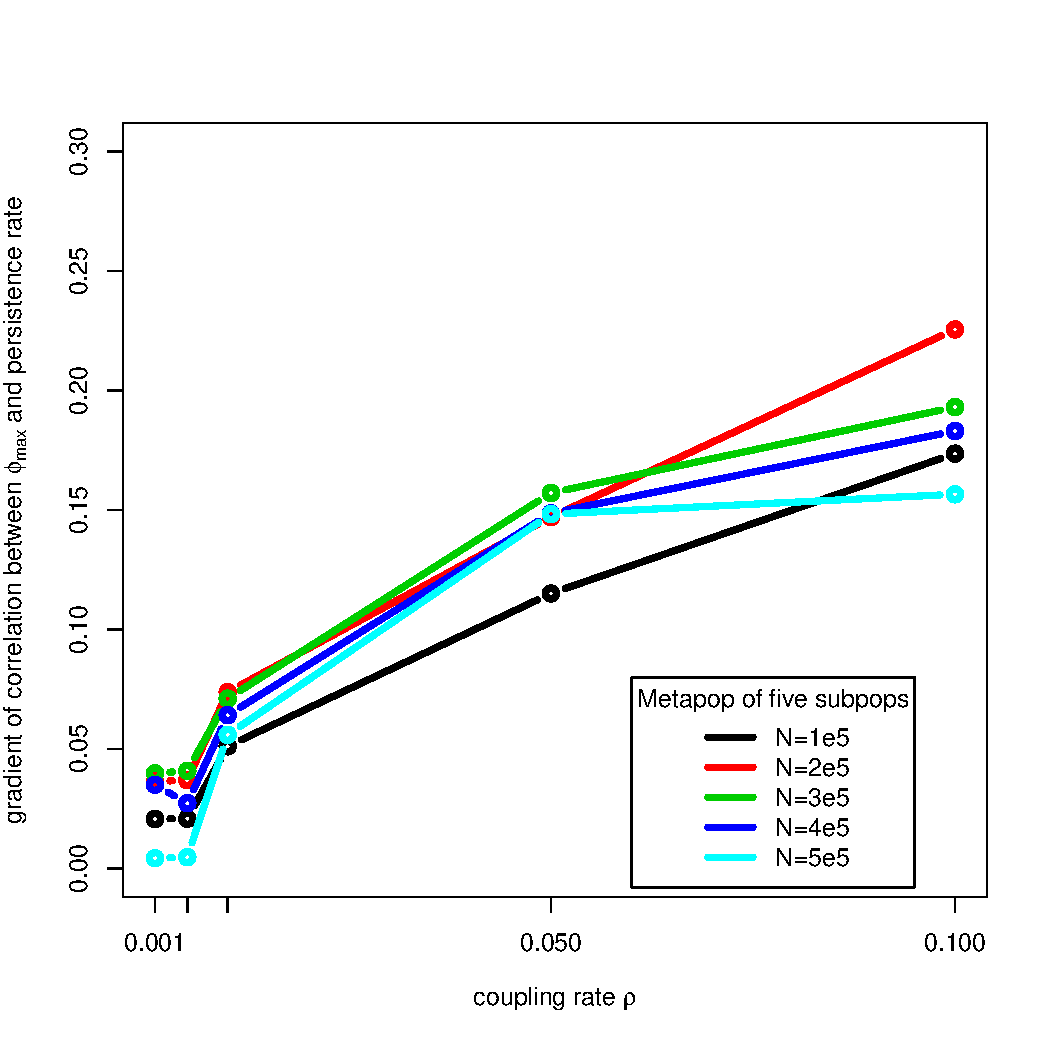
\includegraphics[width=0.5\textwidth]{resVil05RhoChageNchange}
\caption{Correlation between coupling rate and gradient of level of synchrony
and persistence rate in the metapopulation of five subpopulation.
Here, the coupling rate $\rho$ is in \{0.001, 0.005, 0.01, 0.05,
0.1\}, the level of synchrony $\varphi_{max}$ in \{0,$\pi/2$ ,$\pi$\}
and the population size of each subpopulaiton N from$100,000$ to
$500,000$.}


\label{fig:perrateMultVil-1} 
\end{figure}


Due to this result (figure \ref{fig:perrateMultVil-1}), we show that
the coupling rate between subpopulation augments, thus we get an increase
of gradient coefficient. It means that global disease persistence
time in metapopulation strengthens for coupling rate between subpopulations
though how many is population size of subpopulation with the interaction
strength $\rho$ from $10^{-3}$ to 0.1 \cite{KeelingRohani2008}.

Moreover, because of dispersal rate $\rho$, the persistence time
of metapopulation is considered as a function of dispersal rate. In
order to affirm this supposition, here, we permit coupling rate change
from weak to strong in a metapopualtion of five subpopulations with
$N=10^{5}$ for each subpopulation. The dispersal rate $\rho$ is
divised into three intervals. These are low, intermediate and high
coupling rate intervals. In each interval, we choose some coupling
rates that highlight the coupling strength among subpopulations in
a metapopulation. We have the result as follows ( figure \ref{fig:resPenteVil05multiRho-1}).

\begin{figure}[tbph]
\centering 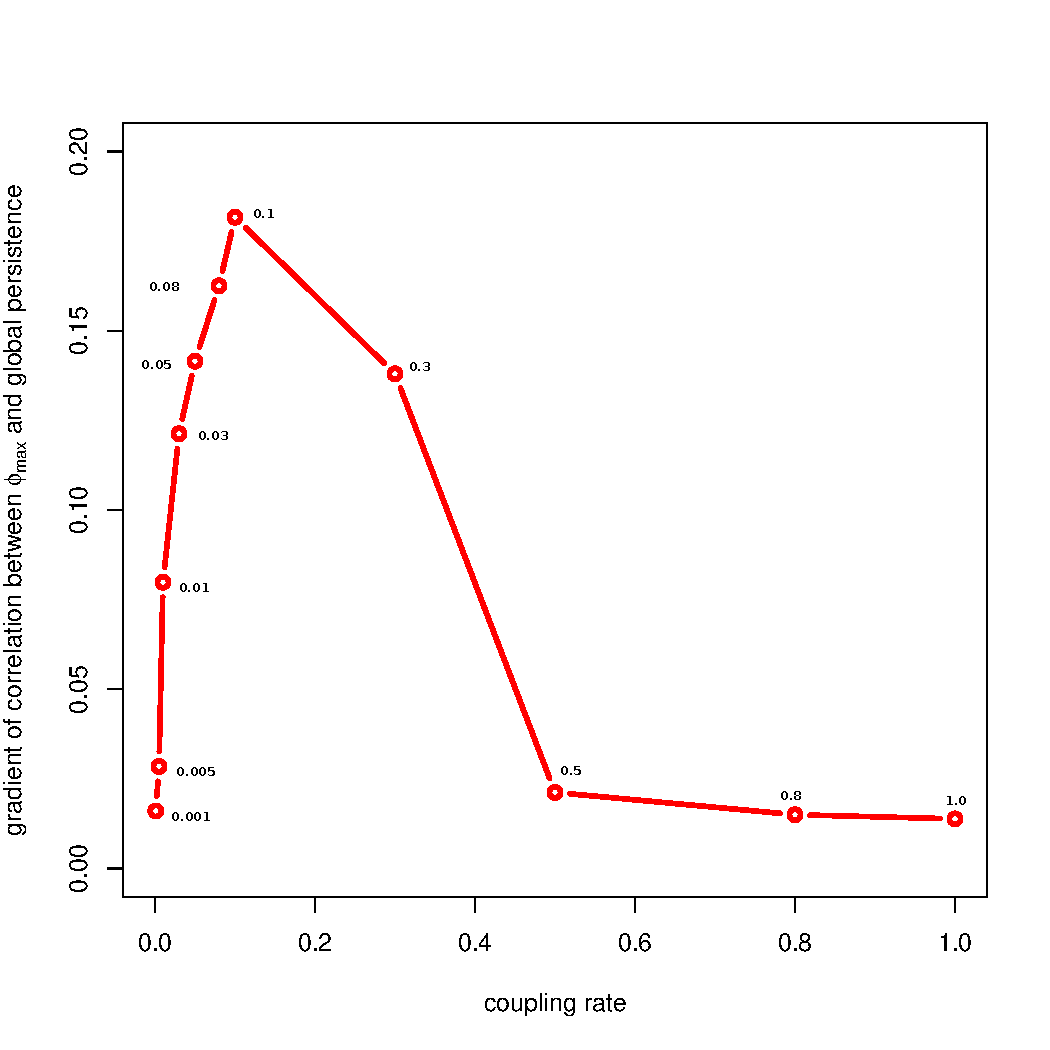
\includegraphics[width=0.5\textwidth]{resPenteVil05multiRho}
\caption{Correlation between coupling rate and gradient of level of synchrony
and persistence rate in the metapopulation of five subpopulation.
Here, the coupling rate $\rho$ is in \{0.001, 0.005, 0.01, 0.05,
0.1, 0.5, 1\}, the level of synchrony $\varphi_{max}$ in \{0,$\pi/2$
,$\pi$\} and the population size of each subpopulaiton N=1e5.}


\label{fig:resPenteVil05multiRho-1} 
\end{figure}


When the coupling rate is small from 0.001 to 0.005, the gradient
of correlation between $\varphi_{max}$ and persistence rate increases
very slowly. However, the persistence rate augments in a sudden way
when the coupling rate changes from 0.005 to 0.1. Lastly, the gradient
strongly decreases when the coupling rate is so robust from 0.5 to
1. Based on this figure, the disease persistence is one humped function
for the coupling rate and the coupling rate is . The medium coupling
rate (from 0.005 to 0.1) maximizes disease persistence in metapopulation.


\section{Conclusion and perspective}

We successfully built a version for the susceptible-infectied-recovered
stochastic metapopulation model. The infection rate $\lambda_{i}$
for \textbf{$subpopulation_{i}$ }portrayed all effects inside as
well as outside on disease tranmission chain between individuals in
the same subpopulation or in other subpopulations. Moreover\textbf{,
}our metapopulation model becames more detailed when we brought seasonality
in metapopulation model to create periodic transmission in year that
here highlights seasonal change as well as school period of children.
We have metapopulation model with different contact rates. This is
more complex model than any used metapopulation model. We sketched
successfully in-phase and sometime out-of-phase (``antiphase'')
models across suburbs of He's 2003 \cite{He2003}.

In order to continue my thesis, we will exploit the global persistence
and the disease transimission among subpopulations under a new shape
of metapopualtion in epidemiology. It is the gravity model in epidemiology.
This model is a very simple model, and can be used to explain the
spatial epidemiologic dynamics. We says it simply that the strength
of coupling between any two populations depends on size of these two
populations and the distance between them (so this model is quite
similar to Newton's law of universal gravitation, the attraction between
two bodies depends on the masses of the bodies and the distance between
the bodies). In epidemiology, we will call the \textquotedbl{}mass\textquotedbl{}
the population size. Then, we set a gravity metapopulation model with
the different positions and the different population sizes of subpopulations.
Finally, we will exploit the disease transmission in the gravity metapopulation
model.

One more main work in my thesis, it is the optimization of the vaccination
policies. We set it in the last part of my thesis, because first of
all, we must deeply exploit the actual nature of the infectious disease
transmission in the different disease model, then we are going to
have a good vaccination policy for a metapopulation

 \bibliographystyle{plain}
\bibliography{bib_art_Pers,bikBokEpidemics,bikCCS}


{[}1{]} http://microbiology.mtsinai.on.ca/faq/transmission.shtml

{[}2{]} http://en.wikipedia.org/wiki/Epidemic\_model 
\end{document}
